\chapter{Benchmark Model}

I am planning to experiment with benchmarking the neural network by performing many training trials by varying number of training data sets to reach the optimal network. Initial weight will be randomly chosen \cite{hamey1991benchmarking}. Comparing the performance of the NN with other classification algorithms also provide a degree of freedom to benchmark our model. In the literature there are many classification domains can be found that perform classification task on KOI dataset: K-nearest neighbors (K-NN) \cite{2011MNRAS.414.2602D}, Naive Bays \cite{feigelson2012}, Random Forests \cite{2015ApJ...806....6M}.

\begin{figure}[!h]
\begin{center}
        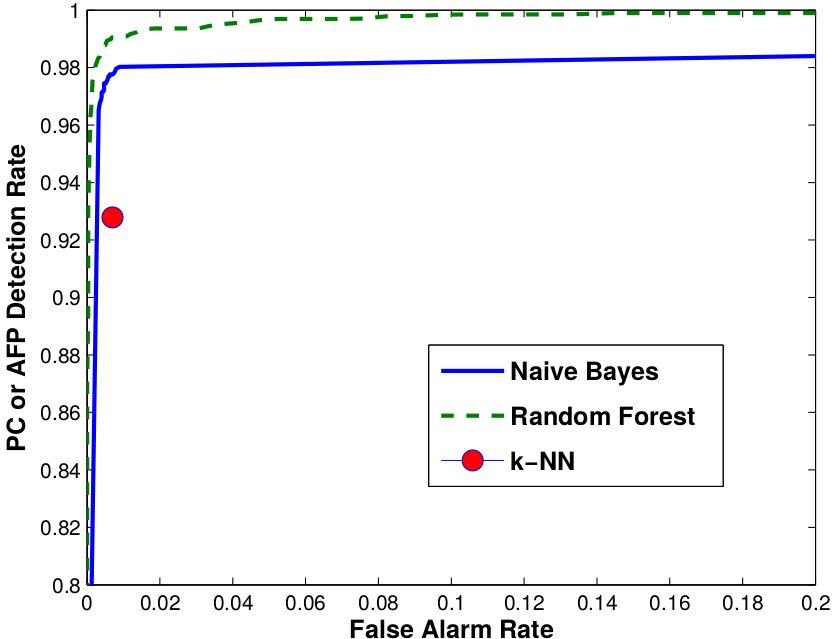
\includegraphics[width=0.35\textheight]{img/benchmark.png}
        \caption{Comparison of Random forest, Naive Bayes and K-NN. Image Credit: McCauliff et al. 2015 \cite{2015ApJ...806....6M}}  \label{fig:benchmark}
\end{center}
\end{figure}

Figure \ref{fig:benchmark} show PC or AFP Detection Rate vs False Alarm Rate of three different classification results performances. K-NN does not produce a ranking of predictions and so is represented as a single point in the plot. The resulting error rates for K-NN and Naive Bays are 3.15$\%$ and 2.73$\%$ respectively. I will be using these statistics that found in the literature as the benchmark for Neural Network using in this project.
